\documentclass{article} 
\usepackage{amsmath} 
\usepackage{amssymb} 
\usepackage{amsthm} 
\usepackage[margin=0.2in]{geometry} 
\usepackage{hyperref} 
\usepackage{physics} 
\usepackage{tikz} 
\usepackage{mathtools}
\usepackage{graphicx}\graphicspath{{./images/}}
\mathtoolsset{showonlyrefs} 
\theoremstyle{definition} 
\newtheorem{theorem}{Theorem}[section] 
\newtheorem{corollary}{Corollary}[theorem] 
\newtheorem{lemma}[theorem]{Lemma} 
\newtheorem{definition}{Definition}[section] 

\author{Connor Duncan}
\date{\today}

\title{notes-10-30-2019}
\begin{document}
\abstract{A single document copy of these notes, as well as a mirror of every note, can be found at \url{connorduncan.xyz/notes}}
\subsubsection{Ex: Soft Sphere Scattering (Altman Returns)} We have some radial potential \begin{equation} V(r)=\left\{\begin{matrix} -V_0 & r<R\\ 0 & r\geq R \end{matrix} \right. \end{equation} where \begin{equation} U(r)=\frac{2mV(r)}{\hbar^2} \end{equation} What's going to happen when we send a low-energy wavevector into this spherical potential? We can write down the radial equation for $\ell=0$ (an $s$-wave). \begin{equation} \left(\pdv[2]{r}+\frac{2}{r}\pdv{r}-U(r)+k^2\right)\psi \end{equation} Take $\xi$ such that \begin{equation} \xi(r)=r\psi(r) \end{equation} where the new wave equation becomes \begin{equation} \left(\pdv[2]{r}-U(r)+k^2\right)\xi(r)=0 \end{equation} This is going to give us a plane wave solution to the schroedinger equation, so we're going to get \begin{equation} \xi(r)=\left\{\begin{matrix} c\sin(kr+\delta_0) &r>R \\ A\sin(Qr) & r<R \end{matrix}\right. \end{equation} \begin{center} 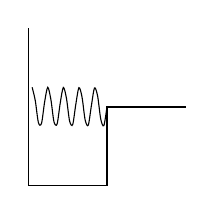
\begin{tikzpicture} \draw (0,2)--(0,0)--(1,0)--(1,1)--(2,1); \draw plot[domain=0:(5*360-90),variable=\x,smooth] ({(\x+90)/(5*360)},{0.25*cos(\x)+1}); \end{tikzpicture} \end{center} We then apply continuity at $R=r$, where $Q=\sqrt{k^2+r^2}$, to get\footnote{note that on the homework, we have a $\delta$ function potential which has different discontinuous boundary conditions at the boundary} \begin{align} A\sin Qr=c\sin(kR+\delta_0) && AQ\cos Qr=ck\cos(kR+\delta_0) \end{align} From this, we're going to end up dividing the two equations by each other to find that \begin{equation} \tan(kR+\delta_0)=\frac{kR}{QR}\tan(QR) \end{equation} Tangent has a lot of divergences though, which makes this equation somewhat challenging to solve. If we assume the argument of $\tan$ is small however, we can taylor expand this to find a close solution to our problem. We'll take $\tan(QR)\sim 1\Rightarrow kR+\delta_0\cong\frac{kR}{QR}\tan(QR)$, so \begin{equation} \delta_0\cong kR\left(\frac{\tan(QR)}{QR}01\right) \end{equation} We can find our scattering length as \begin{equation} a_s=-\lim_{k\rightarrow 0}\frac{\tan(\delta_0)}{k}=-R(\frac{\tan(\gamma R)}{\gamma R}-1) \end{equation} \begin{center} \begin{tikzpicture}[scale=3] \draw (0,2)--(0,0)--(0.5,0)--(0.5,1)--(2,1); \draw[red,thick] plot[domain=0:2*360,variable=\x,smooth] ({(\x)/(360)},{0.25*cos(\x)+1}); \draw[blue,thick] plot[domain=-.2*360:2*360,variable=\x,smooth] ({(\x)/(360)},{0.25*cos(\x-0.2*360)+1}); \draw[red] (2,2)--(2.2,2) node[anchor=west] {Unshifted $\xi$}; \draw[blue] (2,2.2)--(2.2,2.2) node[anchor=west] {Shifted $\xi$}; \end{tikzpicture} \end{center} \paragraph{Scattering Resonances} When $\tan(QR)$ diverges, we're going to have \begin{equation} \tan(kR+\delta_0)+\frac{k}{\gamma}\tan(\gamma R) \end{equation} where $\gamma R\approx\frac{\pi}{2}$. We then have the limit where $k\rightarrow0$, we have that $\delta_0=\pi/2$, so we have a condition. We end up with \begin{equation} \sigma_0=\frac{4\pi}{k^2}\sin^2\delta_0=\frac{4\pi}{k^2} \end{equation} Now, if we want to tune across the resonances, we assume phase shift goes through $\pi/2$ at a certain energy
\end{document}
